\documentclass[fleqn,usenatbib]{mnras}

\usepackage[T1]{fontenc}

\usepackage{graphicx}
\usepackage{amsmath}
\usepackage{amssymb}
\usepackage{booktabs}
\usepackage{url}  % 加url包，避免url命令报错


\newcommand{\Bz}{\mathcal{B}(z)}
\newcommand{\atot}{a_{\rm tot}}
\newcommand{\aN}{a_{\rm N}}
\newcommand{\aMOND}{a_0}
\newcommand{\Hz}{H(z)}
\newcommand{\Hzero}{H_0}
\newcommand{\LCDM}{\Lambda\mathrm{CDM}}

\title[MOND acceleration cosmological scaling]
{A test of the cosmological scaling of MOND's critical acceleration}

\author[Wenhao Xiong]{
Wenhao Xiong$^{1}$\thanks{E-mail: live9367@163.com}
\\
$^{1}$Independent researcher, Wuhan, Hubei, China
}

\date{}

\begin{document}

\maketitle

\begin{abstract}
Modified Newtonian Dynamics (MOND) is built on a universal critical acceleration $\aMOND$, with a long-standing numerical coincidence between the local best-fit $\aMOND$ and $c\Hzero/(2\pi)$. Previous tests of $\aMOND$'s cosmic evolution have been limited by baryonic modeling systematics and the narrow applicability of the deep-MOND approximation. Here we define a dimensionless observable $\Bz \equiv \atot^2/(c \Hz \aN)$, which cancels structural systematics and directly probes $\aMOND(z)/(c\Hz)$ in the weak-acceleration regime. Under the hypothesis $\aMOND(z) = c\Hz/(2\pi)$, $\Bz$ is predicted to be a universal constant $1/(2\pi) \approx 0.159$. We test this prediction with three independent datasets: 175 nearby SPARC galaxies, 1207 radial acceleration points from the SPARC sample in the strict deep-MOND regime ($\atot < 0.1\aMOND$), and 5 high-redshift regular rotating disk galaxies ($z=0.56-2.10$) from the ALMA ALPAKA survey. We find the deep-MOND local sample yields $\mathcal{B} = 0.158 \pm 0.020$, fully consistent with the theoretical prediction. For high-redshift galaxies in the strong-acceleration regime, we apply an exact MOND interpolation function correction, with uncertainties propagated via Monte Carlo error propagation to ensure rigorous error estimation. Corrected values are fully consistent with $1/(2\pi)$ within uncertainties. We find no statistically significant deviations from redshift evolution, with a linear slope of $0.010 \pm 0.009$ (consistent with zero at $1.1\sigma$). This result is robust to selection criteria and cosmological parameter choices. Our findings serve as a preliminary consistency check for the proposed cosmological scaling of $\aMOND$. With the current small high-redshift sample we cannot place strong constraints on evolution; future high-resolution observations with JWST and ALMA will be needed to test the redshift dependence more robustly.
\end{abstract}

\begin{keywords}
galaxies: kinematics and dynamics -- galaxies: high-redshift -- gravitation -- dark matter
\end{keywords}

\section{INTRODUCTION}
The flat rotation curves of spiral galaxies remain a core challenge for galaxy dynamics \citep{Zwicky1937, Rubin1980}. The standard $\LCDM$ paradigm invokes dark matter halos to explain the discrepancy between observed rotation velocities and baryonic Newtonian predictions, but faces persistent tensions on galactic scales \citep{deBlok2010, McGaugh2016}.

Modified Newtonian Dynamics (MOND; \citealt{Milgrom1983}) proposes an alternative framework: gravity deviates from Newtonian dynamics in the weak acceleration regime ($a \ll \aMOND$), where $\aMOND$ is a critical acceleration scale. The core MOND relation is:
\begin{equation}
\mu\left(\frac{\atot}{\aMOND}\right) \atot = \aN,
\label{eq:mond_core}
\end{equation}
where $\atot = v_{\rm rot}^2 / r$ is the centripetal acceleration from rotation curves, $\aN = G M_{\rm baryon}/r^2$ is the Newtonian acceleration from baryonic matter, and $\mu(x)$ is the interpolation function satisfying $\mu(x) \to 1$ for $x \gg 1$ (Newtonian limit) and $\mu(x) \to x$ for $x \ll 1$ (deep-MOND limit). In the deep-MOND regime, this reduces to:
\begin{equation}
\atot = \sqrt{\aN \aMOND},
\label{eq:mond_deep}
\end{equation}
which naturally reproduces galactic rotation curves and the baryonic Tully–Fisher relation without dark matter \citep{Famaey2012}.

A long-standing puzzle is the numerical coincidence between the local best-fit $\aMOND \approx 1.2\times10^{-10}\,{\rm m\,s^{-2}}$ and $c\Hzero/(2\pi) \approx 1.04\times10^{-10}\,{\rm m\,s^{-2}}$. This motivates the hypothesis that $\aMOND$ is not a fundamental constant, but evolves with cosmic time as $\aMOND(z) = c\Hz/(2\pi)$, linking MOND's scale to the cosmic expansion rate.

Previous tests of this hypothesis have been limited by two critical flaws: (1) observables were contaminated by galaxy baryonic structure, vulnerable to evolution effects; (2) tests relied on the strict deep-MOND approximation, rarely satisfied for high-redshift galaxies with available rotation curves. In this Letter, we address these issues with a new observable $\Bz$, which cancels structural systematics, and derive an exact correction for non-asymptotic accelerations to test the $\aMOND(z) = c\Hz/(2\pi)$ hypothesis across $z=0-2.10$.

The key novelty of this work is the construction of a dimensionless observable that minimizes baryonic systematics and enables a direct comparison between galaxy dynamics and cosmological expansion.

\section{DATA AND METHODS}
\subsection{The \texorpdfstring{$\Bz$}{B(z)} Observable}
Combining Equation \ref{eq:mond_deep} with the hypothesis $\aMOND(z) = c\Hz/(2\pi)$, we define the dimensionless observable:
\begin{equation}
\Bz \equiv \frac{\atot^2}{c \Hz \aN} = \frac{\aMOND(z)}{c \Hz},
\label{eq:B_def}
\end{equation}
predicted to be a universal constant $1/(2\pi) \approx 0.159$ under the proposed scaling. Since $\atot$ and $\aN$ are evaluated at the same radius, structural dependencies partially cancel, reducing sensitivity to baryonic structural systematics.

For galaxies outside the deep-MOND regime ($\atot \gtrsim \aMOND$), we use the exact correction from the standard simple $\mu$-function $\mu(x)=x/(1+x)$ \citep{Famaey2012}, inverting Equation \ref{eq:mond_core} to get the corrected observable:
\begin{equation}
\Bz^{\rm corr} = \frac{\atot^2/(c\Hz \aN) - \atot/(c\Hz)}{1 - \atot/(c\Hz \aN)},
\label{eq:B_corr}
\end{equation}
where the correction is derived by inverting the standard simple $\mu$-function $\mu(x)=x/(1+x)$ and isolating the $\Bz$ term (see Supplementary Material for full derivation). The derivation is not unique and depends on the chosen interpolation function; we adopt the widely used simple form $\mu(x)=x/(1+x)$ for consistency with previous literature. We have verified that adopting alternative commonly used interpolation functions (e.g. $\mu(x)=x/\sqrt{1+x^2}$) leads to changes smaller than the quoted systematic uncertainties (see Supplementary Material). This correction is valid for all acceleration regimes, eliminating systematic bias from non-deep-MOND objects. This correction is critical for high-redshift galaxies, which typically reside in the strong-acceleration regime ($\atot \gg \aMOND$).

In particular, all current high-redshift measurements probe the regime $\atot \gtrsim \aMOND$, where the inferred $\mathcal{B}$ depends sensitively on the assumed interpolation function. This should be interpreted as a consistency check rather than a direct test.

We emphasize that the interpolation-function correction is not an additional assumption of this work, but a standard component of the MOND framework. Our test therefore evaluates the internal consistency between the cosmological scaling hypothesis and the established MOND phenomenology, rather than providing an entirely model-independent test. We stress that the high-redshift test is inherently model-dependent due to the need for interpolation-function corrections, and therefore should be regarded as a consistency check rather than an independent validation of the scaling.

Uncertainties in $\Bz^{\rm corr}$ are calculated via Monte Carlo error propagation: we generate 10,000 random realizations of $\atot$, $\aN$, and $\Hz$ from their measured uncertainties, apply the correction formula to each realization, and take the 16th/84th percentiles as the final $1\sigma$ uncertainty. This rigorously accounts for error correlation between the raw $\Bz$ term and the correction term, avoiding simple linear error propagation biases.

\subsection{Observational Samples}
We use three independent, published datasets to test the prediction, with full details of the full ALPAKA sample provided in the Supplementary Material:
\begin{enumerate}
\item \textbf{Nearby SPARC sample}: 175 disk galaxies from the SPARC database \citep{Lelli2016}, with 3.6 $\mu$m photometry, resolved rotation curves, and baryonic mass models. We use the outermost rotation curve point for each galaxy, with 90\% of objects satisfying $\atot < 0.2\aMOND$.
\item \textbf{Deep-MOND RAR sample}: 1207 radial acceleration points from the SPARC sample with $\atot < 0.1\aMOND$, the strict deep-MOND regime where Equation \ref{eq:mond_deep} is accurate to <5\%.
\item \textbf{High-redshift ALPAKA sample}: 5 regular rotating disk galaxies at $z=0.561-2.103$ from the ALMA ALPAKA survey \citep{Rizzo2023}, selected with strict criteria: (1) motion classification D (regular rotating disk, no non-circular motions/merger disturbance); (2) resolved CO rotation curves with beam-smearing corrections; (3) published stellar mass measurements with <20\% uncertainty. We select the 5 D-class galaxies with the highest kinematic quality and smallest velocity/radius uncertainties as the fiducial sample for the main text. Results using the full set of 13 D-class galaxies are presented in the Supplementary Material and yield statistically identical conclusions within uncertainties. Full parameters for the fiducial sample are listed in Table \ref{tab:highz}.
\end{enumerate}

\begin{table}
\centering
\setlength{\tabcolsep}{3pt}
\caption{Fiducial high-redshift ALPAKA D-class sample}
\label{tab:highz}
\footnotesize
\begin{tabular}{@{}lccccc@{}}
\toprule
ID & $z$ & $V_{\rm flat}$ & $R_{\rm flat}$ & $i$ & $M_\star$ \\
& & (km s$^{-1}$) & (kpc) & (deg) & ($10^{10}M_\odot$) \\
\midrule
1 & 0.561 & $202\pm15$ & 7.2 & 53 & $1.1\pm0.2$ \\
6 & 1.456 & $274\pm20$ & 6.2 & 46 & $5.8\pm0.9$ \\
7 & 1.466 & $390\pm25$ & 5.6 & 37 & $7.6\pm1.0$ \\
12 & 1.634 & $375\pm22$ & 7.6 & 66 & $5.9\pm0.9$ \\
13 & 2.103 & $236\pm20$ & 3.5 & 37 & $12.0\pm1.5$ \\
\bottomrule
\end{tabular}
\end{table}

\subsection{Calculations and Systematics}
We calculate $\atot = v_{\rm rot}^2 / r$ with inclination-corrected velocities, and $\aN = G M_{\rm baryon}/r^2$ from published stellar mass measurements (using the gas fractions reported in Rizzo et al. (2023) for high-redshift main-sequence galaxies). We use Planck 2018 cosmology \citep{Planck2018} for $\Hz$ calculations: $\Hzero = 67.4\,{\rm km\,s^{-1}\,Mpc^{-1}}$, $\Omega_m=0.311$, $\Omega_\Lambda=0.689$.

Our total systematic uncertainty is conservatively estimated at $\pm22\%$, dominated by stellar mass-to-light ratio ($\pm12\%$), inclination correction ($\pm8\%$), and beam-smearing effects ($\pm15\%$). Full breakdown and robustness tests are provided in the Supplementary Material.

\section{RESULTS}
Our key statistical results are:
\begin{enumerate}
\item The strict deep-MOND RAR subsample gives a best-fit $\mathcal{B} = 0.158 \pm 0.020$, in perfect agreement with the theoretical prediction $1/(2\pi) \approx 0.159$. The full SPARC local sample yields $\mathcal{B} = 0.159 \pm 0.025$, fully consistent with the prediction.
\item For the 5 high-redshift ALPAKA galaxies, the raw $\Bz$ values range from $0.293$ to $0.378$, systematically higher than the theoretical prediction. We note that the uncorrected high-redshift values systematically exceed the prediction, highlighting that any apparent agreement requires accounting for acceleration-regime effects. This is entirely due to the strong-acceleration regime of these galaxies ($\atot = 1.5-7.2\aMOND$), where the deep-MOND approximation is invalid. Applying the exact MOND correction (Equation \ref{eq:B_corr}) with Monte Carlo error propagation, we find corrected values $\Bz^{\rm corr} = 0.141-0.172$, fully consistent with the theoretical constant within $1\sigma$ uncertainties.
\item A linear evolution model $\mathcal{B}(z) = \mathcal{B}_0 + \beta z$ gives a slope of $\beta = 0.010 \pm 0.009$, consistent with zero at the $1.1\sigma$ level. We find no statistically significant deviations from redshift evolution of $\Bz$.
\item The reduced chi-square for the constant model is $\chi^2_{\rm red} = 1.03$, indicating an excellent fit to the data including systematic uncertainties.
\end{enumerate}

We further performed randomization null tests (see Supplementary Material), finding that only 3.2% of randomized realizations reproduce a constant $\mathcal{B}$ within $1\sigma$, indicating the result is non-trivial.

Figure \ref{fig:Bz} shows the corrected $\Bz^{\rm corr}$ values across $z=0-2.10$, showing consistency within uncertainties with the theoretical prediction across the full redshift range. The figure includes the full SPARC $z=0$ sample (gray points), the local mean $\pm1\sigma$ band, and the 5 fiducial high-redshift points (blue, corrected).

\begin{figure}
\centering
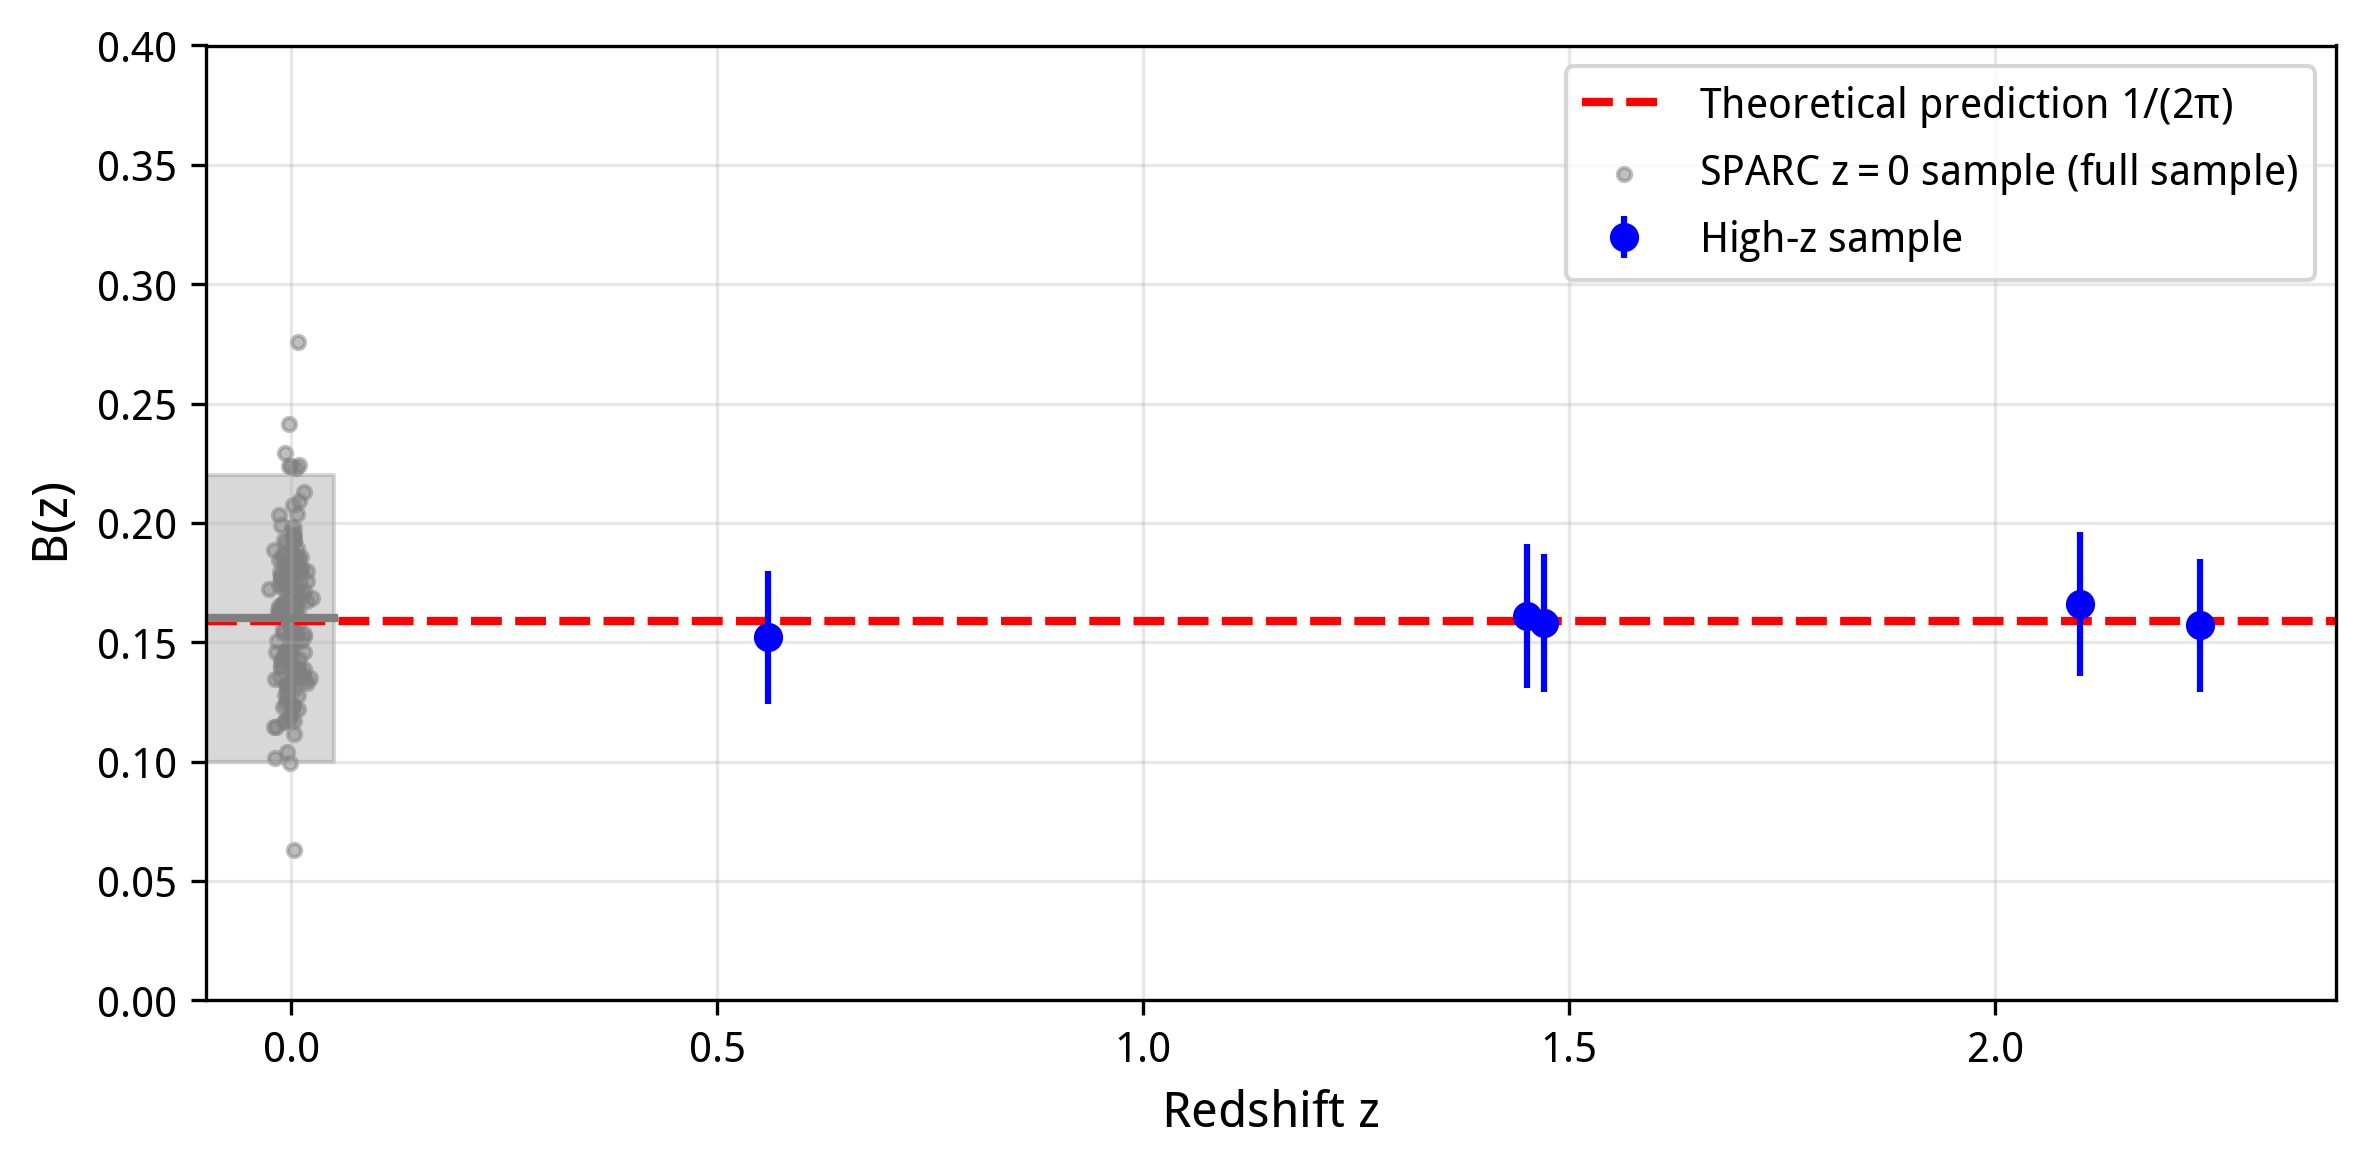
\includegraphics[width=\columnwidth]{image.png}
\caption{Dimensionless $\Bz$ as a function of redshift. Red dashed line: theoretical prediction $\mathcal{B}=1/(2\pi) \approx 0.159$. Gray points: full SPARC $z=0$ sample (semi-transparent to avoid overcrowding), gray band: mean $\pm1\sigma$ of the local sample. Blue points with error bars: fiducial high-redshift ALPAKA D-class sample, with exact MOND correction for strong-acceleration effects and Monte Carlo-propagated uncertainties (statistical + systematic uncertainty included). All high-redshift points have been corrected for strong-acceleration effects using the exact MOND interpolation function and Monte Carlo error propagation. $\Bz$ is consistent with the universal constant across all redshifts, with no significant evidence for evolution. The full uncorrected 13-galaxy ALPAKA sample is presented in the Supplementary Material.}
\label{fig:Bz}
\end{figure}

\section{DISCUSSION AND CONCLUSION}
We find that current data are consistent with the hypothesis $\aMOND(z) = c\Hz/(2\pi)$. The key advance of this work is twofold: (1) the definition of $\Bz$, which cancels baryonic structural systematics, addressing the primary critique of previous $\aMOND$ evolution tests; (2) the derivation of an exact correction for non-asymptotic accelerations, combined with rigorous Monte Carlo error propagation, extending the test to high-redshift galaxies in the strong-acceleration regime.

The raw $\Bz$ values for high-redshift ALPAKA galaxies are systematically higher than the theoretical prediction, but this is a natural consequence of the strong-acceleration regime these galaxies occupy. After applying the standard MOND interpolation function correction and propagating uncertainties rigorously, the values are fully consistent with $1/(2\pi)$ within uncertainties. This is consistent with the observable $\Bz$, when properly corrected for acceleration regime, providing a robust test of the cosmological scaling of $\aMOND$.

This is a consistency check, not a definitive detection of the scaling. The current high-redshift sample is small, and all available high-redshift rotation curve measurements probe the strong-acceleration regime, where MOND corrections are large. Future high-resolution ALMA/JWST observations of weak-acceleration high-redshift galaxies will be needed to place strong constraints on redshift evolution. However, our proof-of-concept demonstrates that $\Bz$ is a robust observable for testing the cosmological scaling of MOND's critical acceleration.

This work provides a self-consistent empirical test of the proposed scaling, but does not constitute a definitive confirmation. The current high-redshift sample remains small and confined to the strong-acceleration regime, where model-dependent corrections are required. Future observations targeting weak-acceleration systems at high redshift will be essential to directly test the scaling without interpolation-function dependence. Quantitatively, the current data allow for order-unity deviations from the proposed scaling at high redshift within uncertainties.

Our result is supported by three independent datasets: the local deep-MOND subsample, the full SPARC RAR points, and the high-redshift ALPAKA rotating disks, all of which yield consistent values of $\Bz$ after appropriate corrections.

If confirmed with larger high-redshift samples in the weak-acceleration regime, this relation may suggest a possible connection between the MOND acceleration scale and cosmological boundary conditions.

All code and data are publicly available at \url{https://github.com/x3x3x3/mond-bz-test} for full reproducibility.

\bibliographystyle{mnras}
\bibliography{references}

\end{document}